% CHAPTER 1
\chapter{WIND TURBINE MODELLING}
\label{chp:3}

\section{VARIABLE SPEED PMSG WIND TURBINES}

The share of variable speed PMSG wind turbines is increasing worldwide due to the high efficiency and torque density. This type of wind turbines are equipped with full-scale power electronics which enable the turbine to have wide speed range. Even though the permanent magnet price fluctuates with time, the reliability and high efficiency of this type of turbine increase its share in the market. \\

 

\begin{figure}[h!]
	\centering
	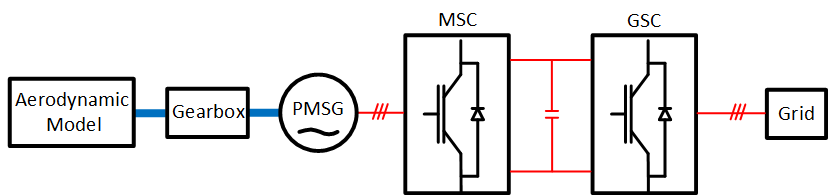
\includegraphics[width=.98\linewidth]{Windmodel.png}
	\caption{Variable Speed Geared Wind Turbine Model}
	\label{varspeedpmsg}
\end{figure} 

Figure \ref{varspeedpmsg} shows the modelling of variable speed wind turbine. The aerodynamic sub-model includes turbine structure that captures power from the wind. The gearbox establishes the connection between wind turbine and PMSG. In this type of wind turbines, PMSG is not directly connected to grid so that the turbine speed is independent from the grid frequency. Therefore, back-to-back converter is used between generator and the electrical grid. The converter which is connected to PMSG is called Machine Side Converter (MSC) meanwhile the one connected to grid is called Grid Side Converter(GSC).

\subsection{Aerodynamic Model}
Aerodynamic model is the sub-model that captures power from the wind. the output of this block is the aerodynamic torque that rotates the turbine. However, the wind speed is not the only input. Turbine speed and pitch angle are also the inputs of the system since they affect the mechanical power that is captured from the wind.

\begin{equation}
P_{WIND}=0.5\rho_{air}\pi R^{2} v^{3}
\label{windpower}
\end{equation}

\begin{equation}
C_{p}(\lambda,\beta)=c_{1}(c_{2}/\lambda_{i}-c_{3}\beta-c_{4})e^{-c_{5}/\lambda{i}}+c{6}\lambda
\label{cp}
\end{equation}

\begin{equation}
\frac{1}{\lambda_{i}}=\frac{1}{\lambda+0.08\beta}-\frac{0.035}{\beta^{3}+1} 
\label{lambdai}
\end{equation}